\documentclass[a4paper, 11pt]{article}

\usepackage[english]{babel}
\usepackage[utf8]{inputenc}
\usepackage[T1]{fontenc}
\usepackage{graphicx}
\usepackage{color}
\usepackage{amsmath,amssymb}
\usepackage{rotating}
\usepackage{layaureo}
\usepackage{booktabs}
\usepackage{varioref}
%\usepackage{subfigure}
\usepackage{listings}
\usepackage{wrapfig}
\usepackage{siunitx}
\usepackage{physics}
\usepackage{subcaption} 
\usepackage{subfloat}
\usepackage{caption}
\usepackage{gensymb}
\usepackage{mhchem}
\usepackage{afterpage}

\sisetup{output-decimal-marker={.}}

\author{Jakub Skowronski \& Alessandro Compagnucci}
\title{GALTRACE: }

\begin{document}

\maketitle

\clearpage

\tableofcontents

\clearpage

\section{Introduction}

One of the modern detection methods, offering identification of the reaction
products with very low energy, is the Pulse Shape Analysis (PSA). This method
can be applied to the signals from silicon detectors. As shown by Mengoni et
al.~\cite{mengoni}, in the case of the TRacking Array for Charged Ejectile (TRACE) array~\cite{mengoni}, consisting
of 200-$\mu$m thick silicon modules and divided in 60 separately read pixels,
the identification of the \ce{^{1,2,3} H} isotopes can be easily obtained.
In addition, the separation between \ce{^3 He} and \ce{4^ He} was also
observed. This proved that the thin detector, with the uniformity guaranteed
by the fine pad segmentation, may provide a good particle discrimination when
the PSA technique is applied.

\bigbreak

The main idea is the reconstruction of the excitation energy of \ce{^19 O},
a neutron-rich nuclei, by the detection of the evaporated protons,
isotropically emitted in the center of mass reference system with an estimated total cross section of about $50$ mb. For this purpose, a segmented light
charged particle array was employed, made of 4$\Delta$E-E telescopes from the
TRACE project~\cite{mengoni}, positioned at backward angles with respect to
the beam direction, coupled to the GALILEO detection system~\cite{galileo}.
If successful, this would allow to investigate the structure of light reaction
products, such as \ce{Be}, \ce{B}, \ce{C}, \ce{N} and \ce{O} by a direct
measurement of their energy, position, mass, and charge.

\bigbreak

This report presents the initial stages of the GALTRACE detector calibration
with 3 peaks from 3 different $\alpha$ source (\ce{^239 Pu}, \ce{^241 Am},
\ce{^244 Cm}), the construction of the electronical chain for the data
acquisition and the development of a Neural Network (NN) model, based on the
Pulse Shape Anlaysis (PSA) of the signal from the detector, in order to
identify the proton and $\alpha$ particles emmited by the daughter nuclei
produced during the experiment. Finally, an initial and brief attempt for the
$\gamma-\gamma$ coincidences identification is presented.

\clearpage

\section{Physical Motivation}

The knowledge of the nuclide chart far from the stabilty valley is one of the
fundamental topics for the nuclear structure studies, as it could hopefully
lead to the comprehension of the nuclear force, which is responsible both for
the abundance of stable nuclei and for weakly bound systems.
Nuclei can be formed in multiple diffrent combinations of protons and neutrons.
However, because of the fundamental forces and symmetries of Nature, not all
combinantions are stable and bound.

\bigbreak

The nuclear landscape show more than $3000$ of nuclei that are expected to be
bound by the strong force. Among these, less than $300$ are stable, while the
others are bound against the emission of protons and neutrons, or against the
$\beta$-decay, in which a proton decays into a neutron (or vice versa). Some
of the unstable nuclei are long-lived and found on Earth, some are produced
experimentally while other thousands, far from stabiity, are still undetected.
Consequently, from the multitude of nuclei that may exist and that could have
been formed i.e.\ in violent stellar explosions, only a very limited number
have been studied.

\bigbreak

\begin{figure}[h]
  \centering
  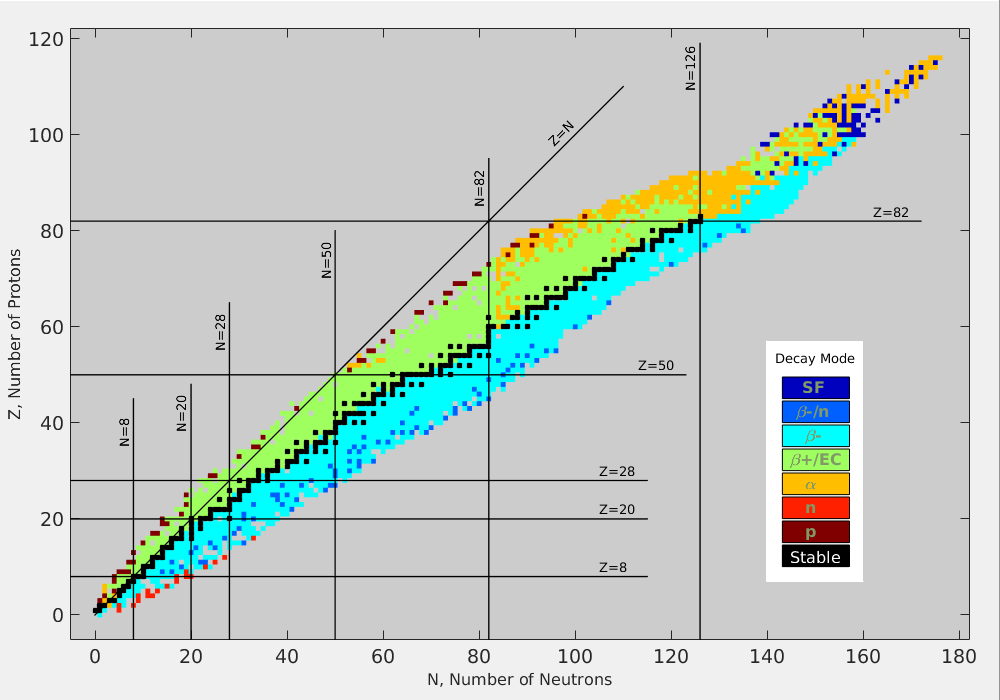
\includegraphics[scale=.35]{img/DecayModeNuDat2.png}
\end{figure}

\bigbreak

In particular, the neutron-rich light isotopes of \ce{Be}, \ce{C}, \ce{O} and
\ce{Ne} offer an extremely fertile ground for nuclear structure studies far
from stabilty region. On one hand, they may serve as examples of nuclear
clustering: for instance, in \ce{^12 C} many states have a well-established
$\alpha$-cluster structure. On the other hand, they exhibit features of
shell-model nuclei in which the impact of the continuum on the shell structure
has to be considered. This characteristics is clearly visible in \ce{^19 O},
in which a comprehensive analysis of the known excitations provides evidence
for states with single-particle structure and states which have strong
$\alpha$-clustering and form rotational bands.

\bigbreak

Description of excitations of the first type involve the standard nuclear
Shell Model (SM), which is an a priori approach; here, the degrees of freedom
are the valence protons and neutrons moving in specific shells – this model
cannot predict cluster states.
The second group of states can be treated with cluster models, which, in turn,
are a posteriori approaches that assume effective building blocks (clusters).
Both these approaches present, however, rather disjointed and not fully
consistent physical descriptions as they assume the nucleus to be a closed
quantum system that is completely isolated from the subspace of scattering and
decay channels. It is clear that a comprehensive understanding of low-energy
excitations in neutron-rich oxygen isotopes cannot emerge from such a picture.

\bigbreak

A significant step forward in creating the link between the SM approach and
the cluster approach to the structure of light nuclei was recently
made~\cite{oko:cluster}~\cite{oko:origin}.
It was showed that the mixing of SM eigenstates, induced by the external
coupling to the decay channel(s), profoundly impacts the nature of SM
eigenstates lying near particle-decay thresholds. 
It was concluded that the mixing of SM eigenstates (with the same quantum
numbers) via the continuum explains:

\begin{itemize}
\item the emergence of clustering leading to the appearance of
collective/cluster states located near the corresponding particle decay
thresholds
\item a gradual disappearance of charged-particle clustering in heavier nuclei
\end{itemize}

The $\alpha$-cluster states, being the best manifestation of the near-threshold
clustering phenomenon, cannot, however, be calculated with the SMEC Model
approach yet. The other class of near-particle-decay threshold states are
states lying close to the nucleon-decay thresholds - they are also
commonly observed in light nuclei. Here, the degree of collectivization can be
predicted by the SMEC Model, but the clear comparison with experiment has not
yet been done. 

\bigbreak

In this context, the measurement of electromagnetic decay from unbound
near-threshold states in neutron-rich systems, which could prove the predicted
near-threshold collectivization phenomenon by the observation of the increase
of electromagnetic transitions probability, would represent a breakthrough.
At present, such information is almost totally missing, as a consequence of
very low  $\gamma$-decay branchings, of the order of $10^{-3}$-$10^{-4}$ and
even lower. The studies call then for the use of very selective reaction
mechanisms and $\gamma$ spectrometers, in order to enhance the sensitivity to
the population of unbound states and their electromagnetic decays.

\clearpage

\section{Experimental Setup}

In order to prepare the data acquistion system, the entire electronical chain
was tested beforehand. In fact it is crucial that the response of each
electronic device used behaves linearly, as the information about the energy
of the incident particle must be univocally extracted at the end of the chain.
To test the PROTO Trace detector, it was put in a vacuum chamber, with a
$\alpha$-ray source.

\clearpage

\section{Calibration results}

In order to prepare the data acquistion system, the entire electronical chain
was tested beforehand. In fact it is crucial that the response of each
electronic device used behaves linearly, as the information about the energy
of the incident particle must be univocally extracted at the end of the chain.
To test the PROTO Trace detector, it was put in a vacuum chamber, with a α-ray
source.

\subsection{Electronical Chain}

\subsection{GALTRACE Linearity}

\begin{figure}[h]
  \centering
  \begin{minipage}[b]{0.45\textwidth}
    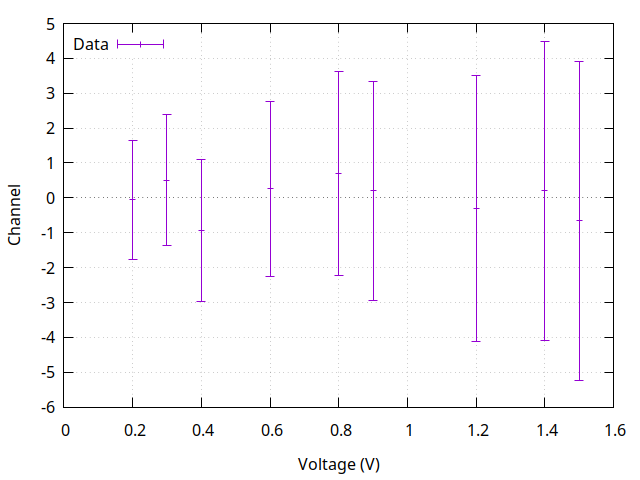
\includegraphics[width=\textwidth]{img/first_board_line/data_2/calib_1.png}
    \caption{Erorr Plot}
    \label{calib:plot:1}
  \end{minipage}
  \hfill
  \begin{minipage}[b]{0.45\textwidth}
  \begin{tabular}{lll}
    Voltage (V) & Channel & $\sigma$ \\
    \midrule
    0.2 & \num{393570.1} & 1.7 \\
    0.3 & \num{393753.2} & 1.8 \\
    0.4 & \num{393934.3} & 2.0 \\
    0.6 & \num{394300.5} & 2.5 \\
    0.8 & \num{394666.1} & 2.9 \\
    0.9 & \num{394848.1} & 3.1 \\
    1.2 & \num{395395.2} & 3.8 \\
    1.4 & \num{395760.8} & 4.3 \\
    1.5 & \num{395942.4} & 4.6 \\
    \bottomrule
  \end{tabular}
  \caption{Data}
  \label{calib:1}
  \end{minipage}
\end{figure}

\subsection{GALTRACE Calibration \& Resolution}

\begin{figure}[h]
  \centering
  \begin{minipage}[b]{0.45\textwidth}
    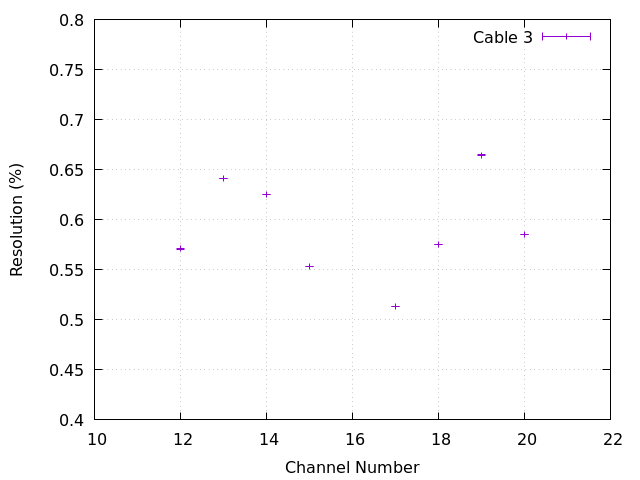
\includegraphics[width=\textwidth]{img/plot/am/3_res_am.png}
    \caption{Resolution vs Channel}
    \label{res:am3}
  \end{minipage}
  \hfill
  \begin{minipage}[b]{0.45\textwidth}
  \begin{tabular}{lll}
    DAQ Channel & Resolution & $\sigma$ \\
    \midrule
    12 & \num{0.5708} & 0.0002 \\
    13 & \num{0.6413} & 0.0003 \\
    14 & \num{0.6253} & 0.0003 \\
    15 & \num{0.5535} & 0.0002 \\
    17 & \num{0.5131} & 0.0002 \\
    18 & \num{0.5752} & 0.0002 \\
    19 & \num{0.6646} & 0.0003 \\
    20 & \num{0.5854} & 0.0002 \\
    \bottomrule
  \end{tabular}
  \caption{Resolution vs Channel plot}
  \label{res:plot:am3}
  \end{minipage}
\end{figure}

\begin{figure}[h]
  \centering
  \begin{minipage}[b]{0.45\textwidth}
    \centering
  \begin{tabular}{ll}
    Channel & FWHM \\
    \midrule
    5150 & \num{29} \\
    5485 & \num{27} \\
    5804 & \num{25} \\
    \bottomrule
  \end{tabular}
  \caption{3-$\alpha$ peaks (cable 1)}
  \label{res:peaks:cab1}
  \end{minipage}
  \hfill
  \begin{minipage}[b]{0.45\textwidth}
    \centering
  \begin{tabular}{ll}
    Channel & FWHM \\
    \midrule
    5153 & \num{32} \\
    5485 & \num{27} \\
    5805 & \num{22} \\
    \bottomrule
  \end{tabular}
  \caption{3-$\alpha$ peaks (cable 2)}
  \label{res:peaks:cab2}
  \end{minipage}
\end{figure}

\clearpage

\section{Data Analysis}

\subsection{ROOT Analysis}

The binary data from the DAQ acquisition was analyzed through a C++ code
implemented in a ROOT framework~\cite{root}.

The Pulse Shape Analysis (PSA) were performed directly on the binary data, as,
by doing thus, it is not necessary to save the signal pulse as a ROOT variable
and a further analysis can be facilitated. The \num{100} ns long stamps of the
signal, saved by the digitizer, were used to obtain two discriminating
variables, that describe fully the important features of the pulse signal for
the proton and $\alpha$ identification: $\tau _{\textup{rise}}$ and
$i_{\textup{max}}$, which represent, respectively, the rise time and maximum
derivative of the signal.

In order to calulcate the two, the following algorithms were used:

\begin{itemize}

\item For the rise time, $\tau _{\textup{rise}}$, the difference between the moment when the pulse is at
  70\%, $t_{0.7}$, and when it is at 30\%, $t_{0.3}$ is considered.
  In order to calculate it, the maximum value of the signal, $V_{\textup{max}}$,
  was obtained as the mean of 3 highest values found. Then, two nearest points
  to 30\% (and 70\%) of the signal were found, in order to perform a two-point
  linear interpolation. Then the $t_{0.3}$ (and $t_{0.7}$) is found from the
  interpolating function as the time when the signal height is at
  $0.3 V_{\textup{max}}$
  (and $0.7 V_{\textup{max}}$).
\item For the maximum derivative of the pulse, $i_{\textup{max}}$, 
  the interpolation of the Pulse Shape was performed using a ROOT class,
  called TSpline3, and 5 highest values of its derivative are used for the
  mean value which is the $i_{\textup{max}}$.

\end{itemize}

\begin{figure}[h]
  \centering
  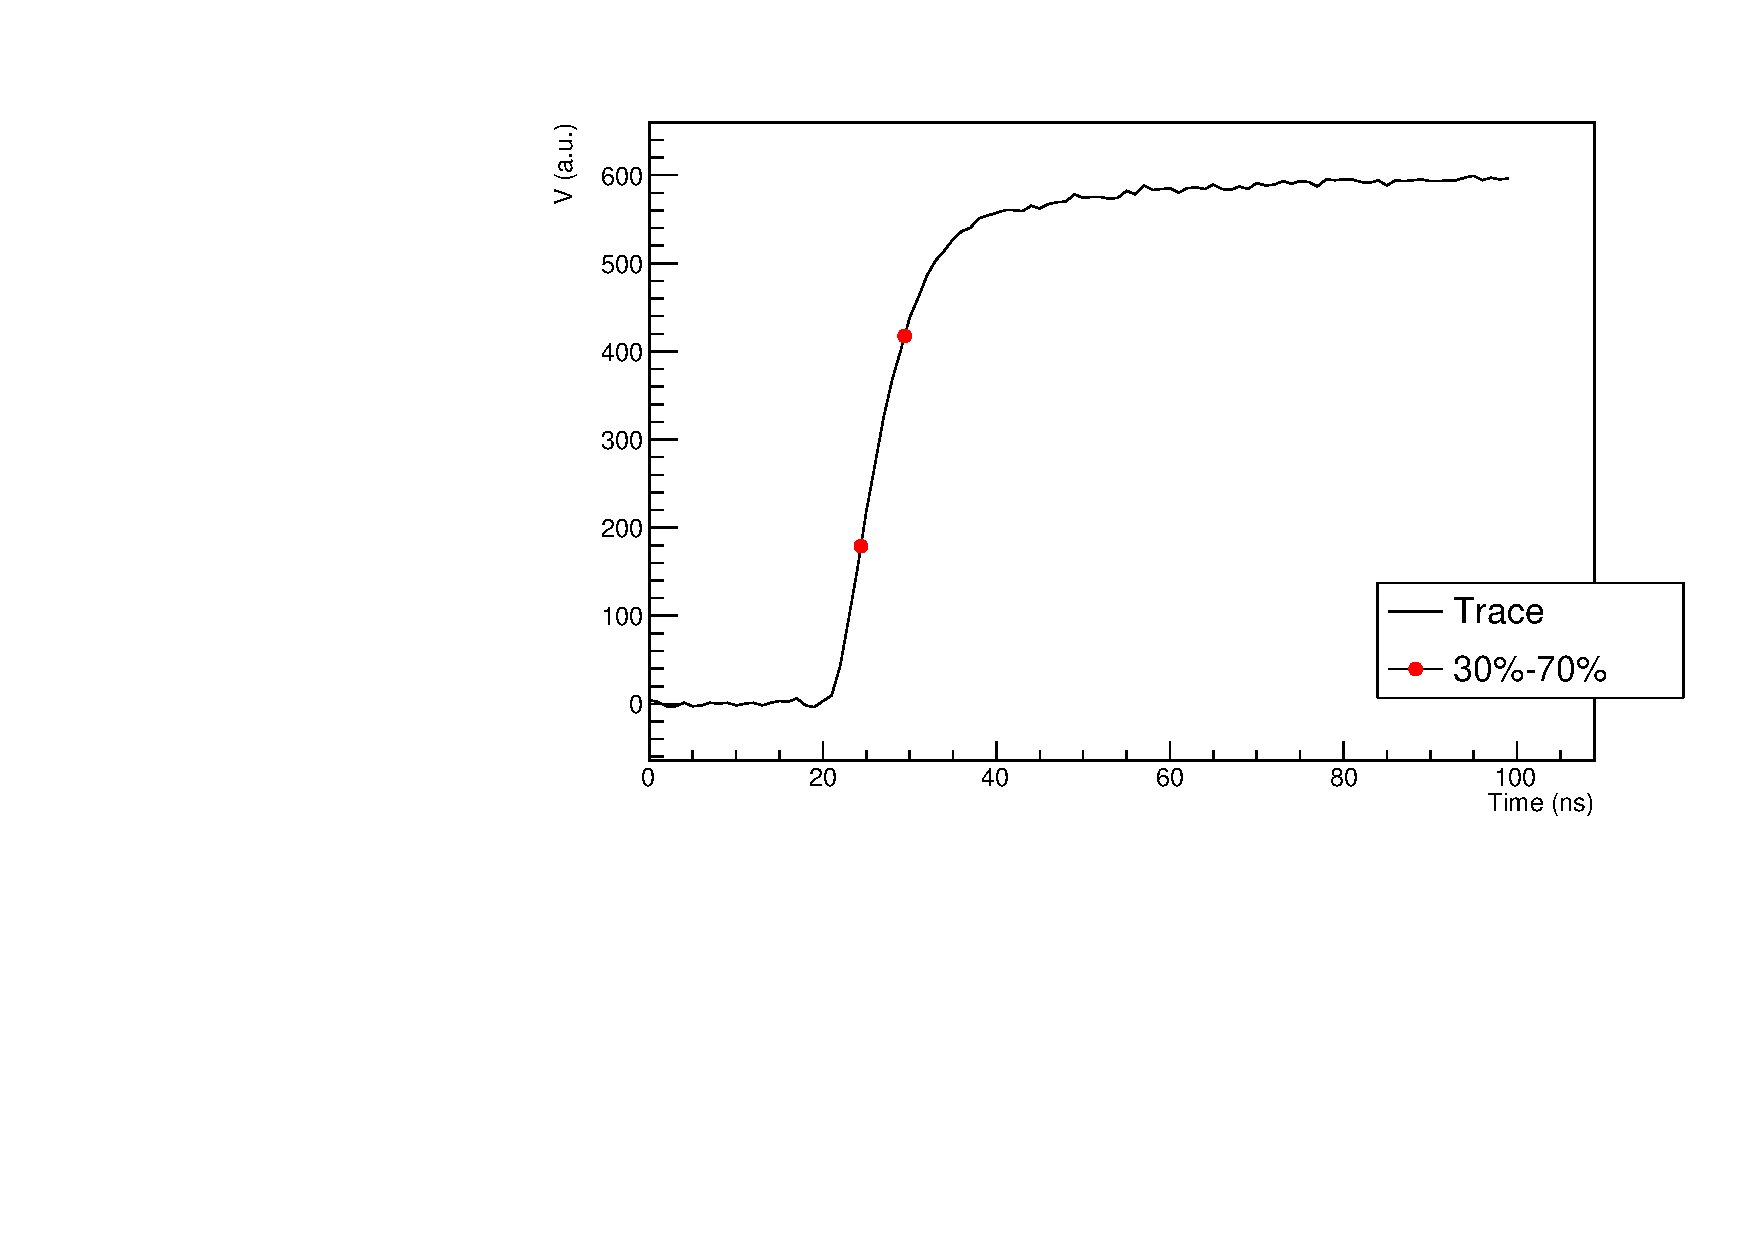
\includegraphics[scale=.6]{img/example_pulse.pdf}
  \caption{An example of the Trace pulse signal. The two points represent the $t_{0.3}$ and $t_{0.7}$.}
  \label{pulse}
\end{figure}

At the end, for each experimental run and each digitizer (the \textit{gal09}
one, and the \textit{gal10}), a TTree object, called \textit{TraceEvent}, was created with the following variables:

\begin{itemize}
\item fDomain
\item fTimeStamp
\item fSubData (vector)
  \begin{itemize}
  \item fSubDomain
  \item fEnergy
  \item fTrace
  \item fTime
  \item fBaseline
  \item fPSA
  \end{itemize}
\end{itemize}
where \textit{fDomain} is the ID of the DAQ used, \textit{fTimeStamp} is the
time given by the digitizer, \textit{fSubDomain} is the detector channel,
\textit{fEnergy} is the energy of the particle and the others are variables
filled according to the PSA: \textit{fTime} is the calculated rise time and
\textit{fTrace} is the maximum derivative of the signal (\textit{fBaseline} and
\textit{fPSA} were later used as Neural Network outputs that gives the
probability of the particle being either a proton or an alpha).

Plots of the $\tau _{\textup{rise}}$ and $i_{\textup{max}}$ in function of the energy
are shown in Fig.~\ref{imax} and Fig.~\ref{risetime}. The $\alpha$ and proton
traces are clearly visible and so they can be tagged and used for the
Neural Network construction. Moreover, even though the signals seem almost
backgroundless, many pulses are present that can not be tagged as neither a
proton nor $\alpha$. In fact, the protons stop at $\approx 4$ MeV and
$\alpha$'s at $\approx 6$ MeV as expected from detector response simulations
performed through LISE software~\cite{lise} (origins of the remaining signals
are not known).

\begin{figure}[h]
  \centering
  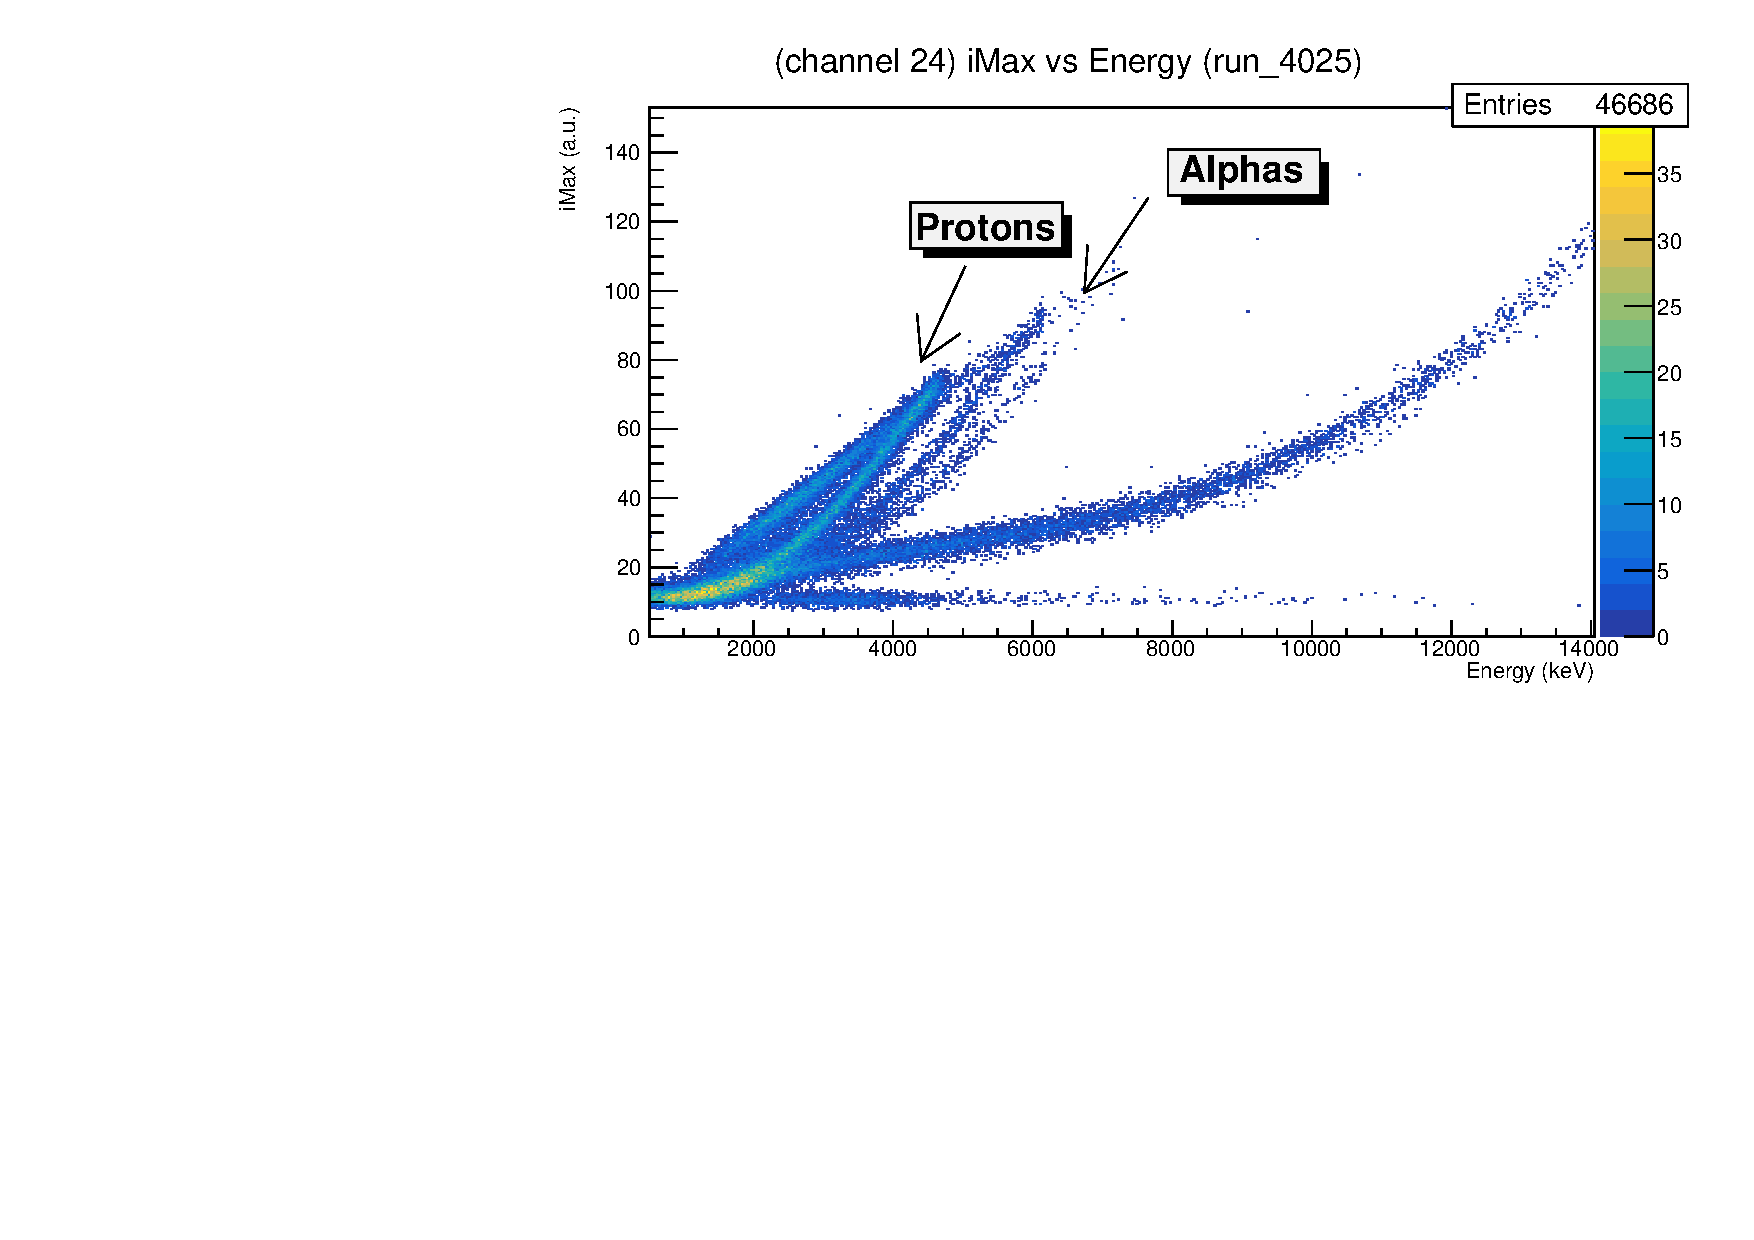
\includegraphics[scale=.6]{img/iMax_4025.pdf}
  \caption{An example of the $i_{\textup{max}}$ vs \textit{E} graph for the 4025 run (only one channel is considered).}
  \label{imax}
\end{figure}

\begin{figure}[h]
  \centering
  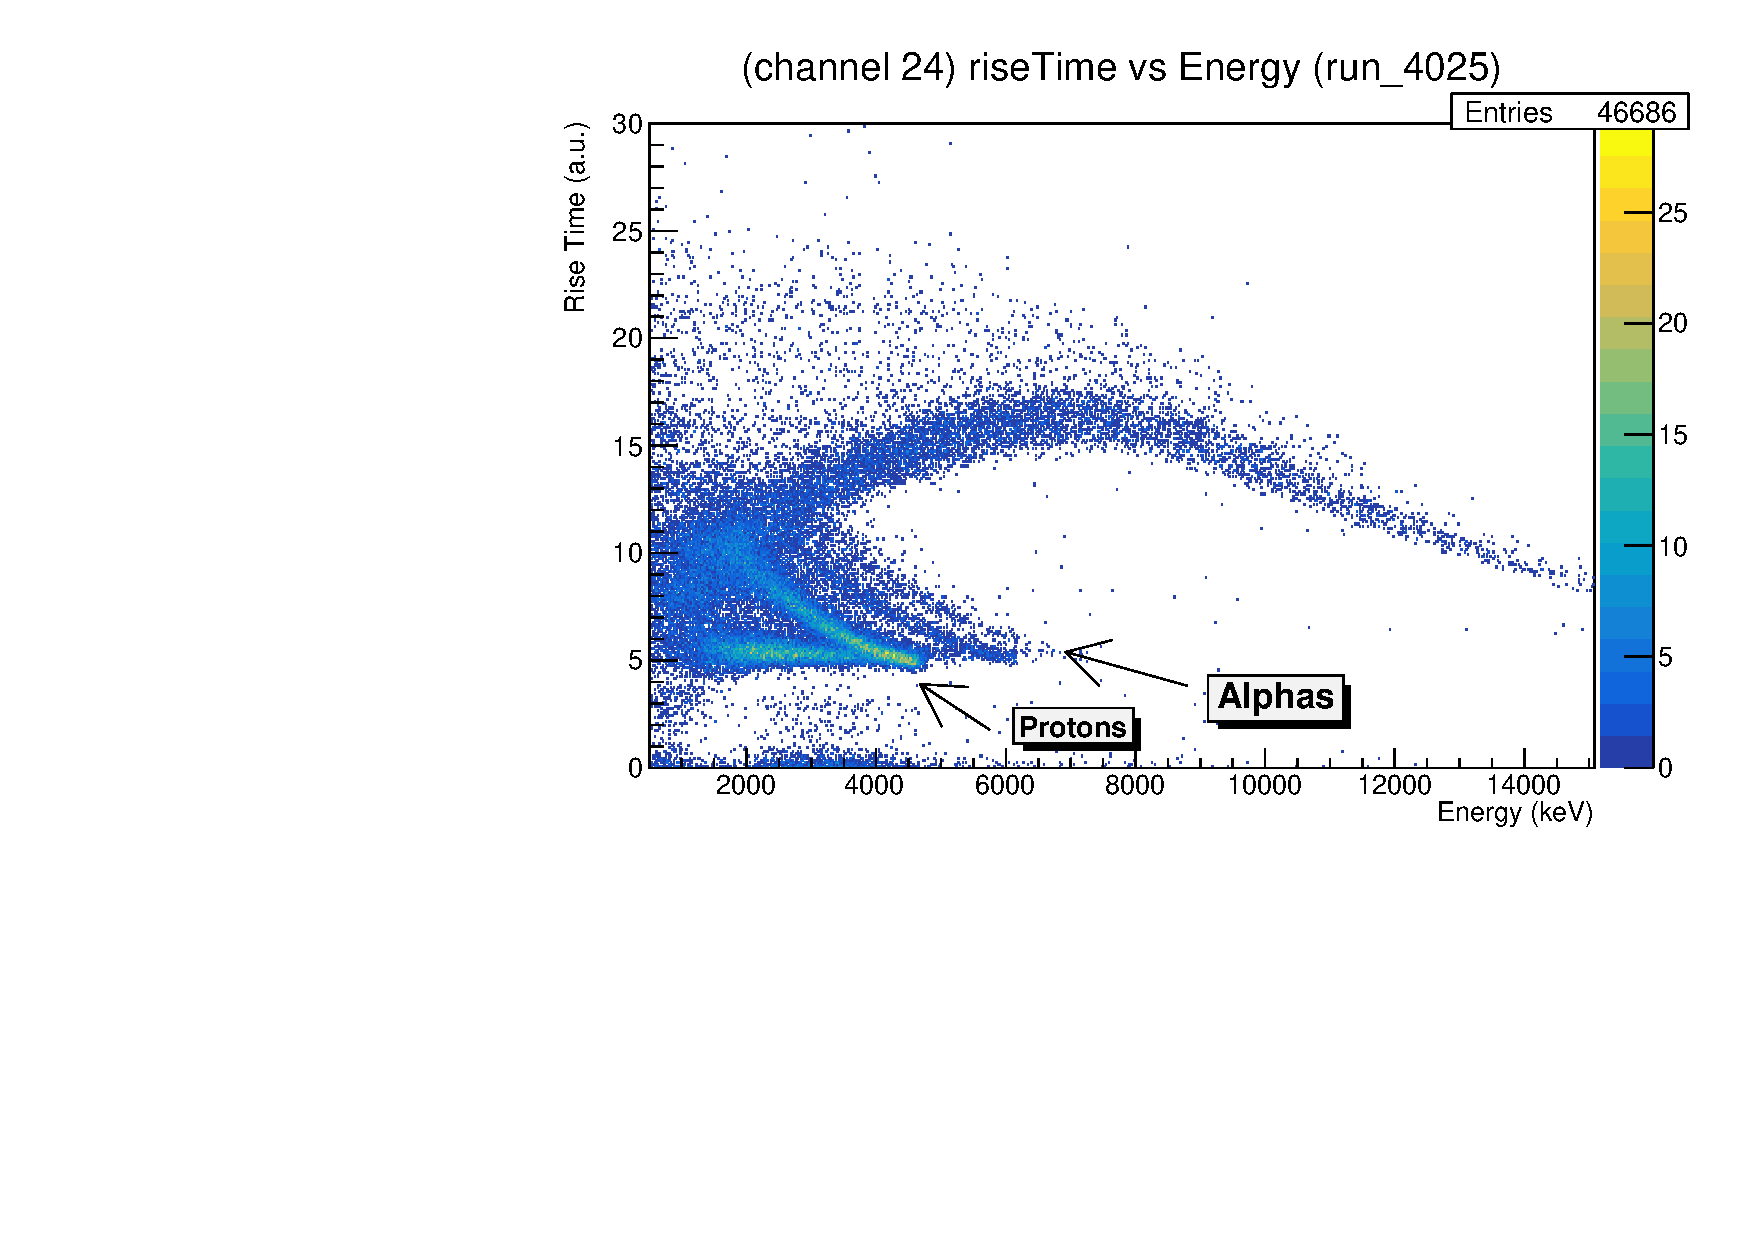
\includegraphics[scale=.6]{img/riseTime_4025.pdf}
  \caption{An example of the $\tau _{\textup{rise}}$ vs \textit{E} graph for the 4025 run (only one channel is considered).}
  \label{risetime}
\end{figure}


\clearpage

\section{Conclusions}

An in-depth characterization and calibration of the TRACE detector was given using an alpha source. The detector was then tested in the GALTRACE experiment at LNL. The data acquired during the different runs was then analyzed in order to reconstruct the structure of each event comprehensive of the PSA variables extracted from the raw signals from the digitizer. Fig.~\ref{imax} and Fig.~\ref{risetime} shows the plot obtained from this analysis.


The also showed that is possible to train a neural network using signals from different regions of the graph to distinguish between different types of particles (Section~\ref{deep}).


A full reconstruction of the events as well as a selection of interesting transition is behind the scope of this work, however some work was made in order to characterize the spectrum obtained by the GALILEO array coupled with the TRACE detector (Section~\ref{gammaspectr}).


\clearpage

\begin{thebibliography}{20}

\bibitem{mengoni}
  D. Mengoni et al.,
  \emph{Digital pulse-shape analysis with a TRACE early silicon prototype}, Nucl. Instrum. Meth. A764 (2014), 241-246.

\bibitem{galileo}
  D. Testov, J.J. Valiente-Dobón, D. Mengoni, F. Recchia, A. Goasduff, A. Boso, S. Lenzi, G. de Angelis, S. Lenzi et al.
  \emph{High resolution $\gamma$-ray spectroscopy using GALILEO array}, arXiv:1903.01296.
  
\bibitem{oko:cluster}
  J. Okolowicz, M. Ploszajczak and W. Nazarewicz,
  \emph{On the origin of nuclear clustering}, Prog. Theor. Phys. Supplement 196 (2012) 230.

\bibitem{oko:origin}
  J. Okolowicz, M. Ploszajczak and W. Nazarewicz,
  \emph{Toward understanding the microscopic origin of nuclear clustering}, Fortschr. Phys. 61, 66 (2013).

\bibitem{mengoni2}
  D. Mengoni,
  \emph{TRACE: a highly-segmented Silicon detector for light charged particles emitted in fusion-evaporation and direct reactions}.
  
\bibitem{strano}
  E. Strano et al., Nucl. Instrum. Methods, B317 (2013) 657.
  

\bibitem{salathe}
Salathe, Marco, and Thomas Kihm. 
\emph{Optimized Digital Filtering Techniques for Radiation Detection with HPGe Detectors}, Nucl. Instrum. Meth. A808 (2016): 150–155.

\bibitem{kuba:compa}
S. Capra, G. Benzoni, A. Compagnucci, J. M. Deltoro, J. Duenas, A. Goasduff, D. Mengoni, A. Pullia, J. Skowronski, I. Zanon, S. Ziliani, 
\emph{Validation and Charcterization of the GALTRACE Silicon Detector Array Demonstrator}.

\bibitem{tensorflow}
Martín Abadi, Ashish Agarwal, et al.
\emph{TensorFlow: Large-scale machine learning on heterogeneous systems},
2015. Software available from tensorflow.org.

\bibitem{pytorch}
Adam Paszke, Sam Gross et al.
\emph{Automatic differentiation in PyTorch},
2017

\bibitem{ml4phys}
Mehta, Pankaj et al. 
\emph{A High-Bias, Low-Variance Introduction to Machine Learning for Physicists.}, Physics Reports 810 (2019): 1–124. Crossref. Web.

\bibitem{baldi}
Baldi, Pierre, Peter Sadowski, and Daniel Whiteson, \emph{Searching for exotic particles in high-energy physics with deep learning}, Nature communications 5 (2014), 4308.

\bibitem{williams}
  Williams, J. Michael. \emph{Machine Learning in HEP}, No. LHCb-TALK-2015-338. 2015.

\bibitem{root}
  Rene Brun and Fons Rademakers,
  \emph{ROOT - An Object Oriented Data Analysis Framework}, Proceedings AIHENP'96 Workshop, Lausanne, Sep. 1996, Nucl. Inst. \& Meth. in Phys. Res. A 389 (1997) 81-86.

\bibitem{lise}
  O.B. Tarasov and D. Bazin,
  \emph{LISE++ : Exotic beam production with fragment separators and their design}, NIM B 376 (2016) 185.

\bibitem{github-nn}
  J. Skowronski \& A. Compagnucci,
  \emph{Neural Network code for GALTRACE particle discrimination} (2019), Github repository, \url{https://github.com/Alecompa/galtrace-nn}

\bibitem{charge:amp}
  A. Pullia and S. Capra,
  \emph{Experimental performance of a highly-innovative low-noise charge-sensitive preamplifier with integrated range-booster}, Journal of Instrumentation 13 (12), art. no. C12004, 2018.

\bibitem{bicmos}
  \emph{The Ams Website}, \url{https://ams.com/}

\end{thebibliography}


\end{document}
